\chapter{Analyse und Auswertung}
\label{ch:analysis}

Im folgenden werden \emph{Gitterdaten} (engl. lattice data) analysiert, wie im Abschnitt \ref{subsec:latticedata} eingeführt. 
Die räumliche Information liegt diskret in Form einer Regionenvariable $s$ vor.  


%\begin{figure}[ht!]
%    \begin{center}
%    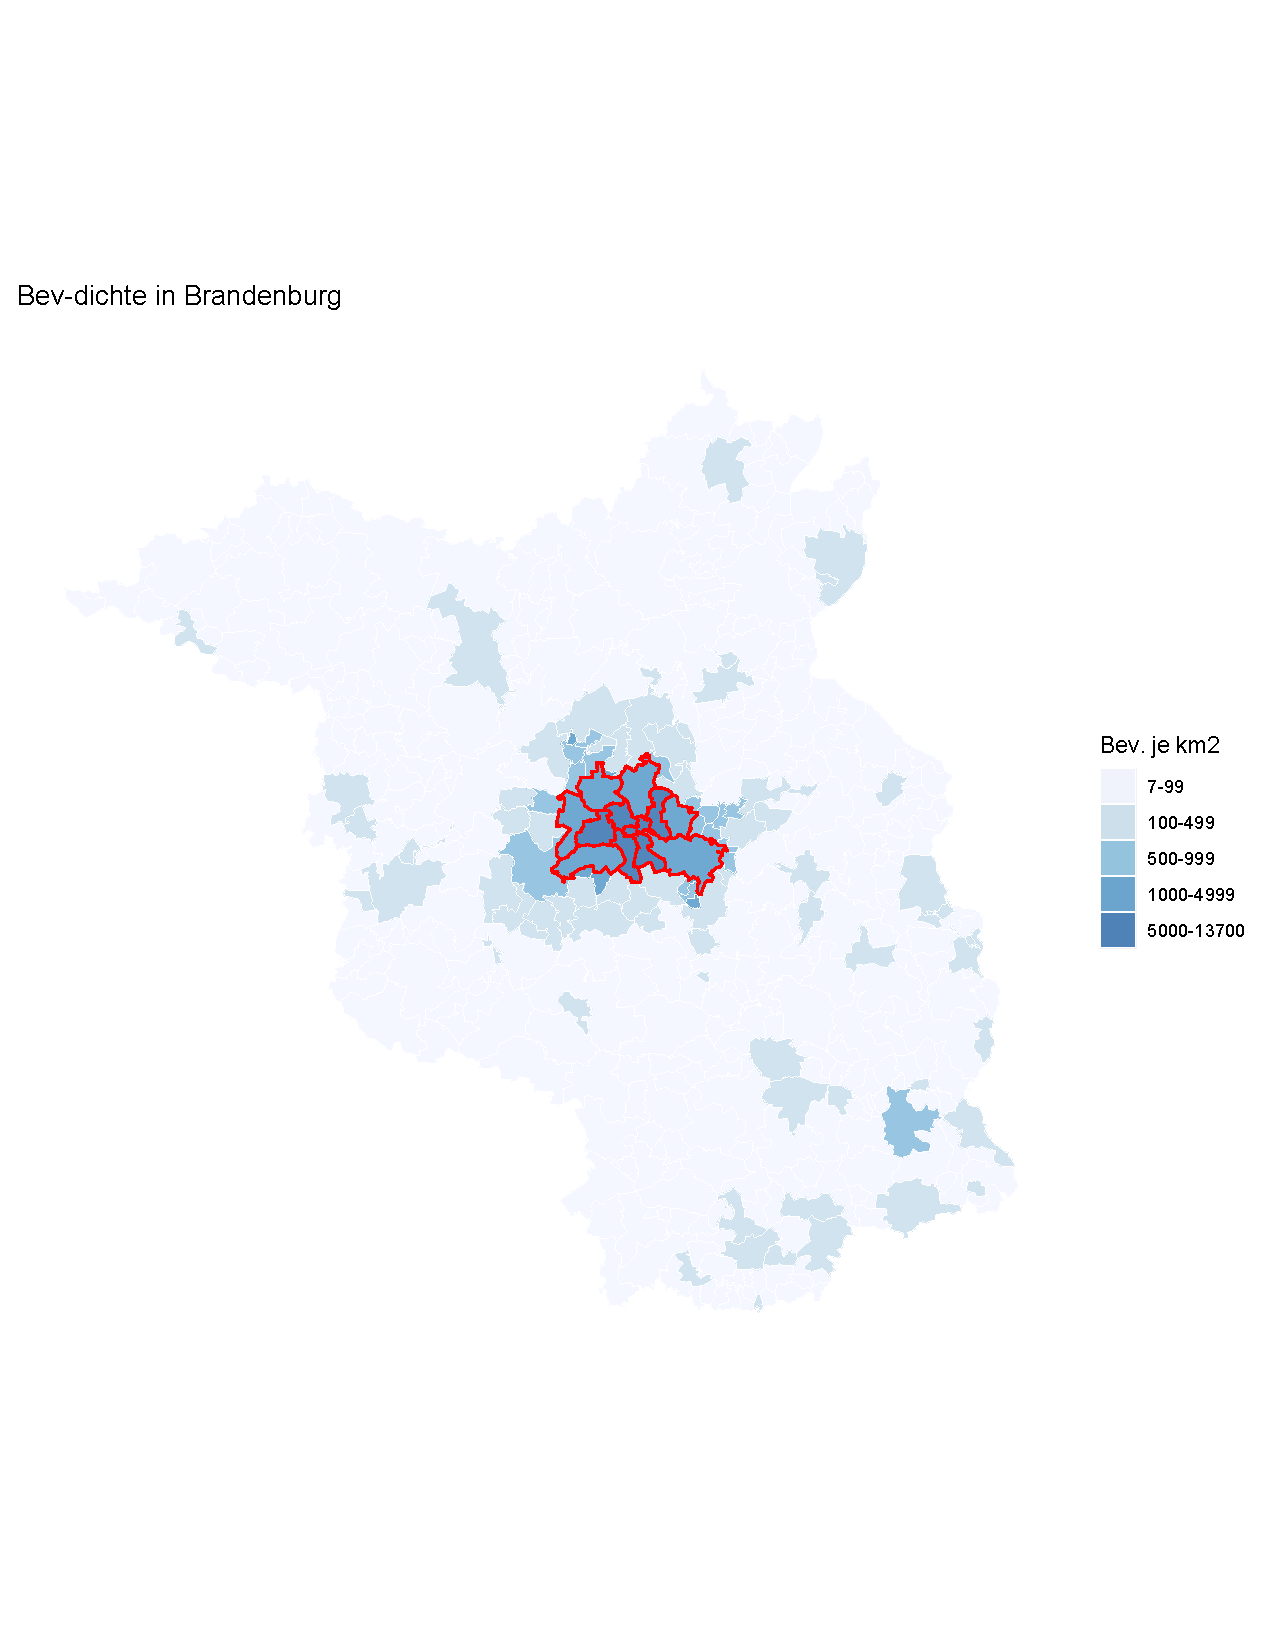
\includegraphics[scale=0.5]{body/figures/Gem-2.pdf}
%    \end{center}
%    \caption[Bevölkerungsdichte in Berlin und Brandenburg]{Bevölkerungsdichte in Berlin und Brandenburg im Jahre 2013. Weitere Details hier eingeben. Grafik erstellt mit Daten aus: Quelle}
%    %Source:
%    \label{fig_bb1}
%   \end{figure}
    

\section{Charakterisierung des Beobachtungsgebietes}

Das Beobachtungsgebiet zeichnet sich durch große Heterogenität der Raumeinheiten bezüglich vieler Merkmale aus. 
Viele Gemeinden sind großräumig abgegrenzt und weisen einen Bruchtteil der Einwohner aus den kleinflächigen, 
dicht besiedelten Berliner Bezirken auf. 
Die Raumeinteilung ist somit wenig einheitlich in der Fläche, 
welche selbst autokorreliert ist.
Die dünn besiedelten ländlichen Gemeinden des Brandenburger Umlandes werden zunächst ignoriert.

Die Anzahl der Lagereimitarbeiter wird geschätzt und liegt aggregiert auf Gemeindeebene vor. 
Exakte Unternehmensstandorte oder Adressdaten sind nicht vorhanden.

Die Bevölkerung auf Ebene der Gemeinden wird durch statistische Schätzungen der Ämter jährlich aktualisiert 
fortgeschrieben und durch einen Zensus alle 10 Jahre überprüft und für die Zukunft angepasst. 
Der nächste Zensus ist für 2021 angesetzt. Distanzen zwischen Gemeinden werden über Zentroide gemessen.

\subsection{Quantilkarten ausgesuchter Attribute}

Wir definieren zunächst Nachbarschaften der Gemeinde-Polygone und nutzen die Queen-Definition: 
Angrenzende Polygone welche mind. 1 Knoten teilen (queen=TRUE) stehen in räuml. Beziehung

%\hspace*{4mm} Gegeben $ \bm{x^{(t)}}=(x_{1}^{(t)},\ldots,x_{p}^{(t)} ) $ in Iteration $t$ , generiere $ \bm{x^{(t+1)}}$:
%\setlength{\parskip}{0pt}

 Als Teilgebiet wird die Metropolregion Berlin-Brandenburg betrachtet. 
 Alle Zentroide im Umkreis von 13 km des eigenen Zentroids einer Region werden als Nachbarn deklariert.
 Jedem Nachbarschaftspolygon wird ein Gewicht zugewiesen. style="W" weist jedem Nachbarn identische Gewichte zu (1/Anzahl Nachbarn). 
 Reihenstandardisierung bewertet Beobachtungen mit wenigen Nachbarn stärker. 
 Problematischerweise haben Randgebiete tendenziell weniger Nachbarn und ihre lag-Werte basieren auf weniger Polygonen. 
 Sie sind somit anfälliger für Über- oder Unterschätzung der tatschlichen Autokorrelation. Hierfür gibt es robustere Alternativen.

 \begin{figure}[!ht]
        \setlength{\abovedisplayskip}{0pt}
        \setlength{\belowdisplayskip}{0pt}
        \setlength{\abovedisplayshortskip}{0pt}
        \setlength{\belowdisplayshortskip}{0pt}
    \centering %Bilder mittig statt am linken Rand ausgerichtet
    \begin{minipage}[b]{.45\linewidth} % [b] => Ausrichtung an \caption --> c (=Center) t (=Top) und b (=Bottom)
        % \linewidth entspricht hier \textwidth (=Breite Textbereich)
        %\centering
        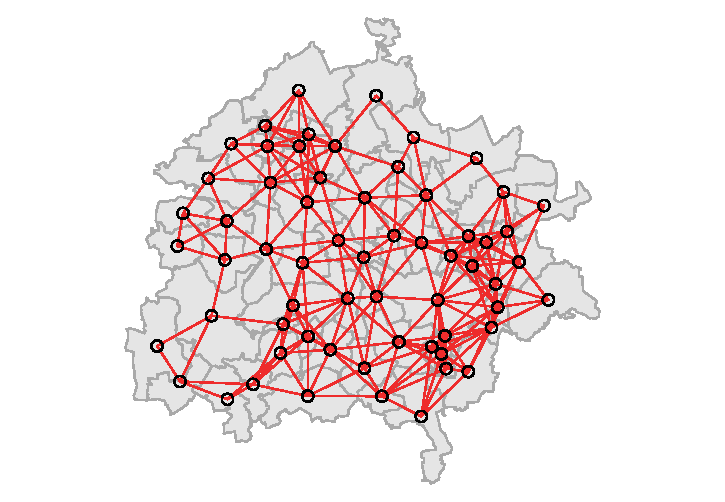
\includegraphics[scale=0.8,trim={0.5cm 0.2cm 0.5cm 0.2cm},clip]{body/figures/analysis/metropol-13km-neighbours.pdf}% [scale=0.5] oder [width=\linewidth]
       %[width=\textwidth] entspricht [width=\linewidth] (=Breite einer Minipage)
       %\caption{emp-bev}
    \end{minipage} % <- sonst wird hier ein Leerzeichen eingefügt
    \hfill
    %\hspace{.1\linewidth}% Abstand zwischen Bilder
    \begin{minipage}[b]{.45\linewidth}
        %\centering
        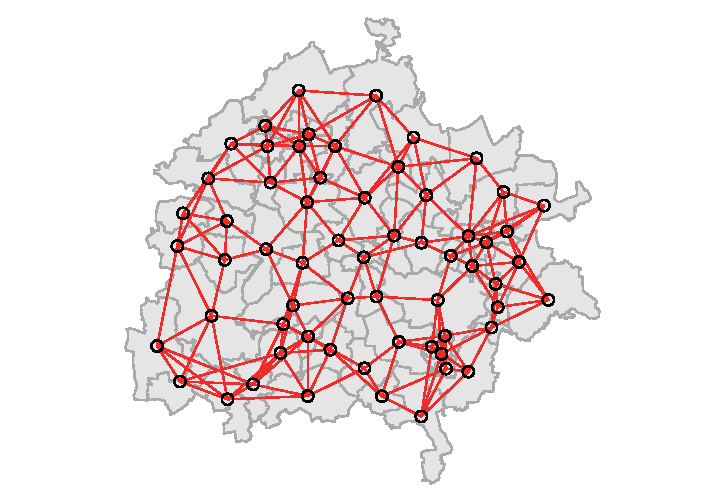
\includegraphics[scale=0.8,trim={0.5cm 0.2cm 0.5cm 0.2cm},clip]{body/figures/analysis/metropol-5-neighbours.pdf}% [scale=0.5] oder [width=\linewidth]
       %\caption{km2}
    \end{minipage}
       %Source:
    \caption[Nachbarschaftsrelationen der Metropolregion]{Nachbarschaftsrelationen: Li: 13km Radius. Re: 5 nächste Zentroide. }
    \label{fig_metropol_neighbours}
\end{figure}

Diese Nachbarschaftsinformationen fließen direkt in die Nachbarschaftsmatrix $W$ ein.
Einige Pakete realisieren dies auch als Nachbarschaftsliste. 

Als mögliche Attribute zur Realisierung der $Y$-Matrix stehen verschiedene Merkmale zur 
Verfügung, welche später auch in die Regression einfließen. Zur explorativen Analyse 
nutzen wir in Abbildung \ref{fig_metropol_y} das \emph{tmap}-Paket, welches die automatische Einteilung 
per Quantil-Klassifikationsschema anbietet.


\begin{figure} %[htb] %h=here, t=top, b=bottom, p=page of float
    \centering %Bilder mittig statt am linken Rand ausgerichtet
    \begin{minipage}[b]{.45\linewidth} % [b] => Ausrichtung an \caption --> c (=Center) t (=Top) und b (=Bottom)
        % \linewidth entspricht hier \textwidth (=Breite Textbereich)
        %\centering
       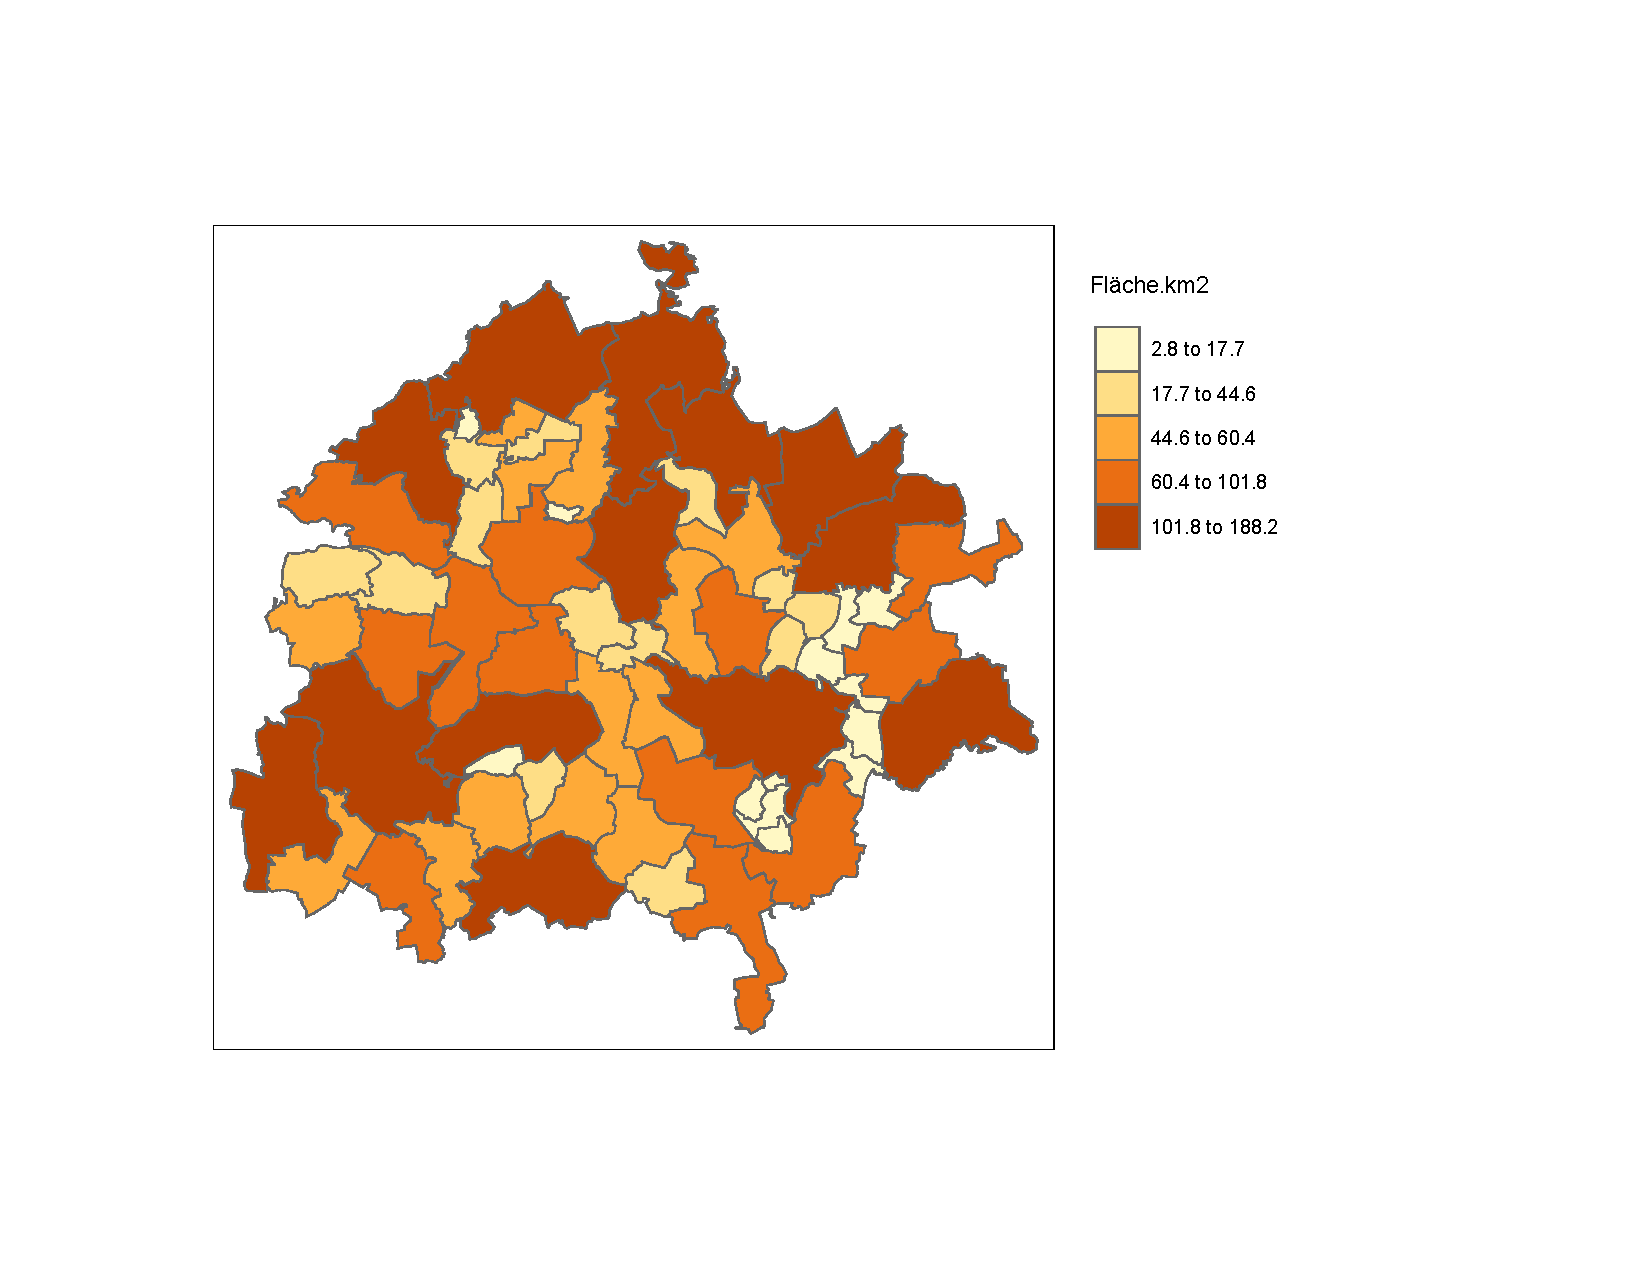
\includegraphics[scale=0.4,trim={1cm 2cm 1cm 2cm},clip]{body/figures/km2.pdf} % [scale=0.5] oder [width=\linewidth]
       %[width=\textwidth] entspricht [width=\linewidth] (=Breite einer Minipage)
       %\caption{emp-bev}
    \end{minipage} % <- sonst wird hier ein Leerzeichen eingefügt
    \hfill
    %\hspace{.1\linewidth}% Abstand zwischen Bilder
    \begin{minipage}[b]{.45\linewidth}
        %\centering
        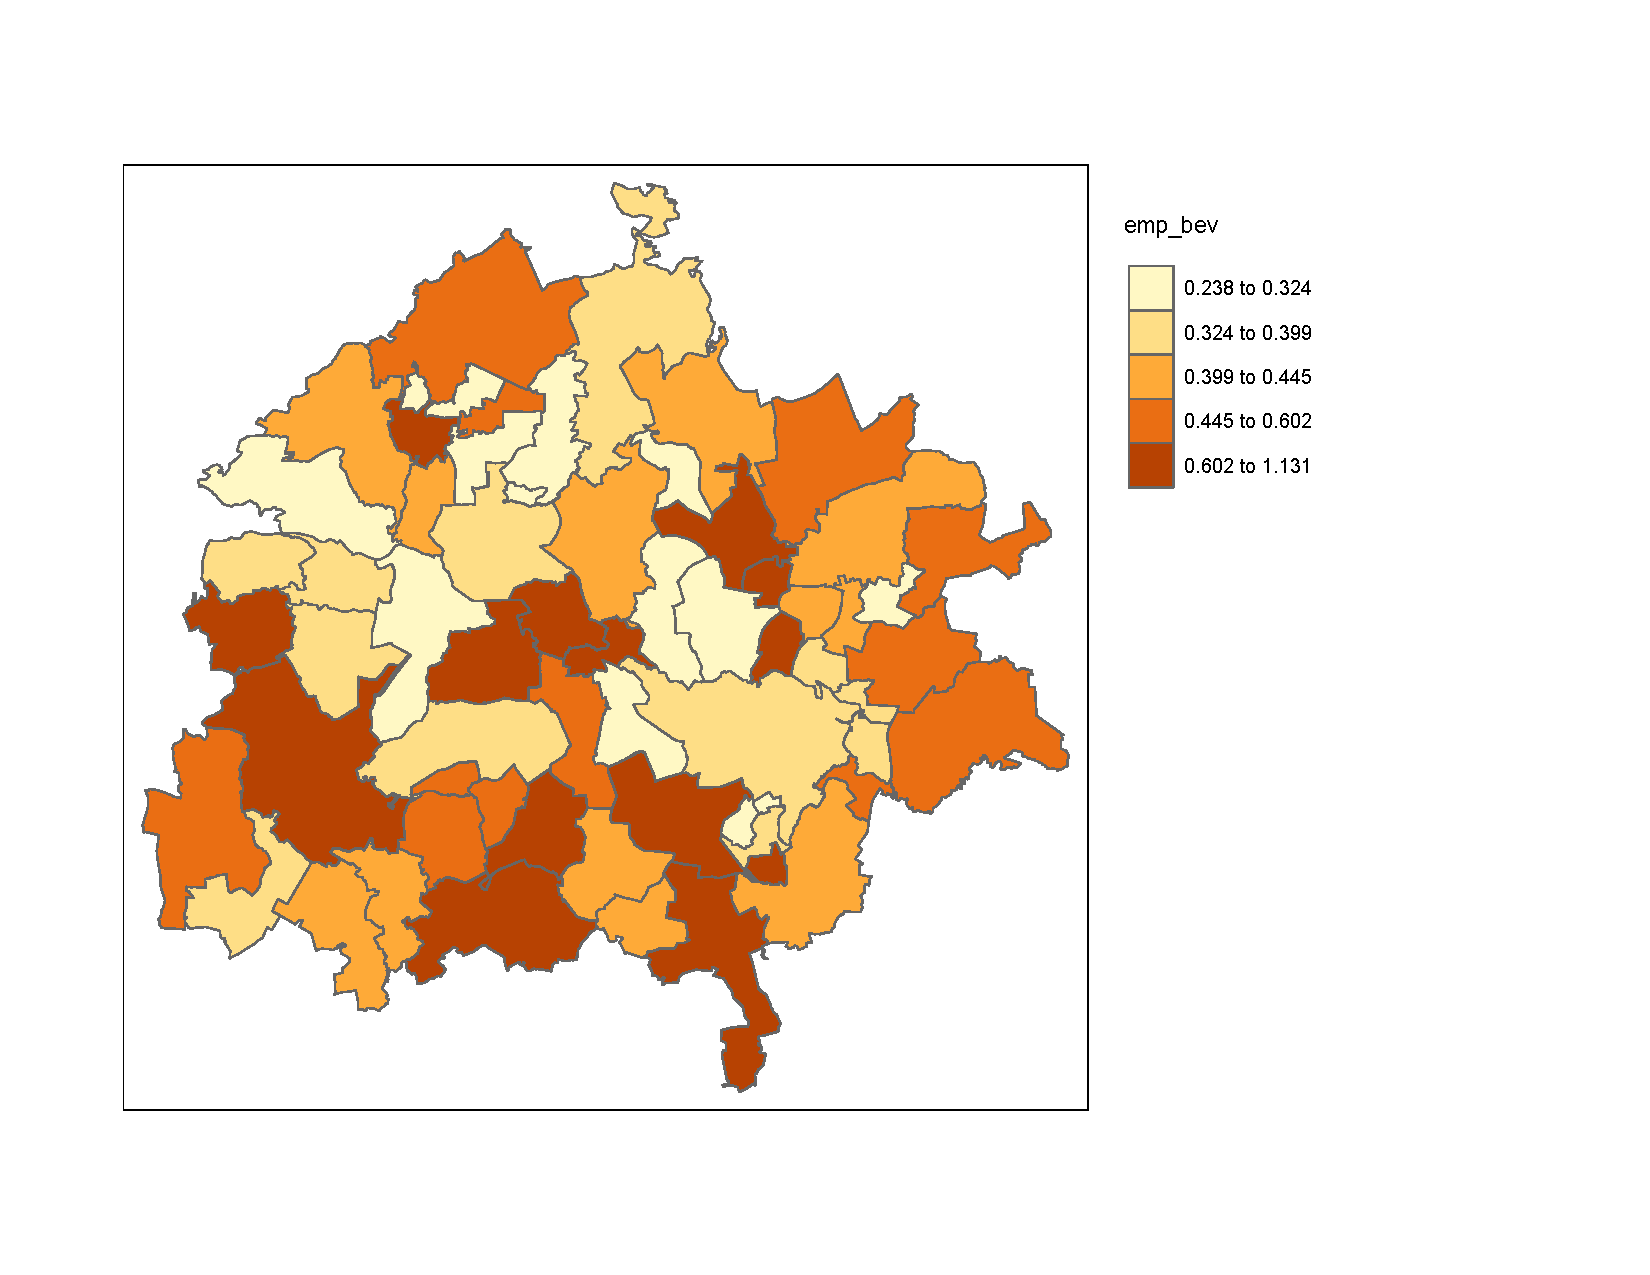
\includegraphics[scale=0.36,trim={1cm 2cm 1cm 2cm},clip]{body/figures/emp-bev.pdf} % [scale=0.5] oder [width=\linewidth]
        %\caption{km2}
    \end{minipage}
    \caption{Quantilkarten der Metropolregion. Li: Fläche Re: Arbeitnehmer je Bev.}
    \label{fig_metropol_y}
 \end{figure}

Zugleich sollen die Verteilungseigenschaften der \emph{Arbeitnehmer per Einwohner} geprüft werden.

%[Histogramme und Kolmogorov-smirnoff]

 \begin{figure}[!ht]
        \setlength{\abovedisplayskip}{0pt}
        \setlength{\belowdisplayskip}{0pt}
        \setlength{\abovedisplayshortskip}{0pt}
        \setlength{\belowdisplayshortskip}{0pt}
        \begin{center}
        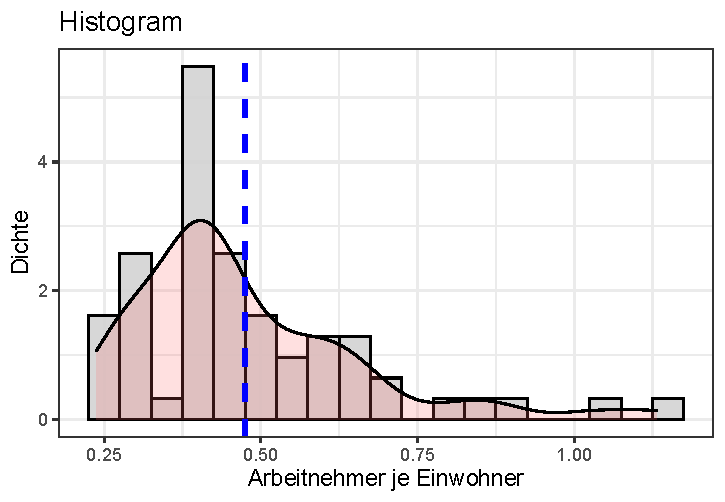
\includegraphics[scale=0.8,trim={0.1cm 0.1cm 0.1cm 0.1cm},clip]{body/figures/analysis/Hist-emp_bev.pdf} % [scale=0.5] oder [width=\linewidth]
            %trim={links unten rechts oben}    
    \end{center}
    \caption[Histogramme ausgewählter Attribute]{Histogramme, emp. Dichte und Mittelwert }
    \label{fig_metropol_hist}
\end{figure}

Eine Normalverteilung scheint für dieses Attribut nicht gegeben. 
Insbesondere Ausreißer großer Werte verzerren die Verteilung. Dies betrifft etwa
die beiden Gemeinden Schönefeld und Großbeeren, in denen nach Datenlage 
mehr Menschen arbeiten als leben. Hierfür müssen Transformation oder Ausreißerbereinigung durchgeführt werden
\section{Globale Indizes}
\label{ch:analysis-GISA}

\subsection{Globaler Moran Index}
Der Standard Morantest unter der Normalverteilugnsannahme entspricht dem Morantest der Regressionsresiduen eines Modells, welches lediglich mit einem Intercept ausgestattet wird. 
Dies zeigt, dass zusätzliche Kovariablen eingeführt werden können, um Missspezifikationen auszubügeln. 
Mit der gleichen Konstruktion kann zudem eine Sattelpunkt-Appriximation statt der analytischen Normalverteilungsannahme (Tiefelsdorf 2002) 
sowie exakter Tests verwendet werden.  %(Tiefelsdorf, Hepple, Bivand)
Diese Methoden sind jedoch numerisch aufwendig, für moderate Datensätze wie im vorliegenden Fall jedoch noch praktikabel. 
Wie die Anwendung in Kapitel 4 zeigt, sind die Unterschiede für globale Tests gering, insbesondere falls Anzahl an Lokationen nicht klein ist. 
Für lokale Maße sind die Unterschiede zwischen Normalverteilungsannahme und Sattelpunktapproximation und exaktem test hingegen ausgeprägter \cite[S. 280]{bivand_applied_2013}.

\begin{lstlisting}[language=R]
    > moran.test(DF$emp_bev,listw = lw, randomisation=TRUE)
# Output:
	Moran I test under randomisation

data:  DF$emp_bev       weights: lw    

Moran I statistic standard deviate = 0.16349, p-value = 0.4351
alternative hypothesis: greater
sample estimates:
Moran I statistic       Expectation          Variance 
     -0.007611493      -0.016393443       0.002885485
\end{lstlisting}

Es gilt $\text{p-value} > \alpha = 0.05$. Die Nullhypothese kann nicht abgelehnt werden und 
es wird keine Autokorrelation erkannt. Die Sattelpunktapproximation liefert ähnliche Werte.

\begin{lstlisting}[language=R]
    > lm.morantest.sad(lm(emp_bev ~ 1,SPDF),listw = lw)
# Output
	Saddlepoint approximation for global Moran's I (Barndorff-Nielsen formula)

Saddlepoint approximation = 0.24664, p-value = 0.4026
alternative hypothesis: greater
sample estimates:
Observed Moran I 
    -0.007611493 
\end{lstlisting}

Der exakte Test liefert:
\begin{lstlisting}[language=R]
    > lm.morantest.exact(lm(emp_bev ~ 1,SPDF),listw = lw)

Exact standard deviate = 0.24433, p-value = 0.4035
alternative hypothesis: greater
sample estimates:
[1] -0.007611493
\end{lstlisting}
Der Geary-Test liefert:
\begin{lstlisting}[language=R]
    > geary.test(SPDF$emp_bev,listw = lw, randomisation=TRUE)

	Geary C test under randomisation

data:  SPDF$emp_bev 
weights: lw 

Geary C statistic standard deviate = -0.1539, p-value = 0.5612
alternative hypothesis: Expectation greater than statistic
sample estimates:
Geary C statistic       Expectation          Variance 
      1.009477840       1.000000000       0.003792393
\end{lstlisting}




\subsection{Monte-Carlo Simulation}

\begin{lstlisting}[language=R]
    > set.seed(1234)
    > MC<- moran.mc(SPDF$emp_bev, listw = lw, nsim=999)
# Output
	Monte-Carlo simulation of Moran I

data:  SPDF$emp_bev 
weights: lw  
number of simulations + 1: 1000 

statistic = -0.0076115, observed rank = 585, p-value = 0.415
alternative hypothesis: greater
\end{lstlisting}

Zur Abschätzung der Signifikanz randomisieren wir die Attributs-Werte über alle 
Gemeinden und implementieren keinerlei räumliche Autokorrelationsstruktur.
Zu jeder Permutation wird ein Regressionsmodell angepasst und der Regressionsanstieg 
als Wert einer Moran I Statistik erfasst.
Die Verteilung aller Werte gibt uns die erwartete Verteilung unter Annahme der Nullhypothese aus, 
dass Attributs-Werte zufällig über die Gemeinden verteilt sind.
Letztlich wird der tatsächliche Moran I-Wert mit der simulierten Verteilung verglichen.

\begin{lstlisting}[language=R]
    n <- 1599L   # Define the number of simulations
    I_r <- vector(length=n)  # Create an empty vector

for (i in 1:n){
  # Randomly shuffle income values
  x <- sample(SPDF$emp_bev, replace=FALSE)
  # Compute new set of lagged values
  x.lag <- lag.listw(rwm, x)
  # Compute the regression slope and store its value
  M_r    <- lm(x.lag ~ x)
  I_r[i] <- coef(M_r)[2]
}
\end{lstlisting}

\section{Lokale Indizes}
\label{ch:analysis-LISA}

\subsection{Lokaler Moran Index}
Je stärker der lokale Moran Index vom Erwartungswert abweicht und je größer der Z-Score bzw. je kleiner der p-Value sind, 
desto unwahrscheinlicher ist die Annahme von nicht autokorrelierten, zufallsverteilten Daten.

\begin{figure}[!ht]
    \setlength{\abovedisplayskip}{0pt}
    \setlength{\belowdisplayskip}{0pt}
    \setlength{\abovedisplayshortskip}{0pt}
    \setlength{\belowdisplayshortskip}{0pt}
\centering %Bilder mittig statt am linken Rand ausgerichtet
\begin{minipage}[b]{.48\linewidth} % [b] => Ausrichtung an \caption --> c (=Center) t (=Top) und b (=Bottom)
    % \linewidth entspricht hier \textwidth (=Breite Textbereich)
    %\centering
    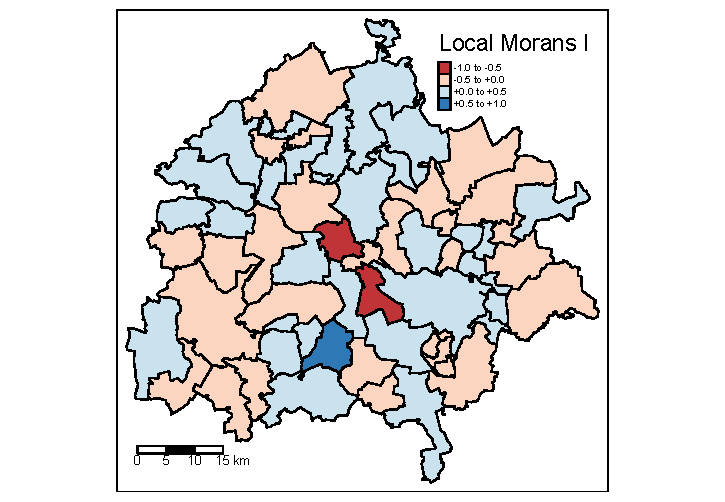
\includegraphics[scale=0.75,trim={0.2cm 0.1cm 0.2cm 0.1cm},clip]{body/figures/analysis/metropol-LMI.pdf}% [scale=0.5] oder [width=\linewidth]
   %[width=\textwidth] entspricht [width=\linewidth] (=Breite einer Minipage)
   %\caption{emp-bev}
\end{minipage} % <- sonst wird hier ein Leerzeichen eingefügt
\hfill
%\hspace{.1\linewidth}% Abstand zwischen Bilder
\begin{minipage}[b]{.48\linewidth}
    %\centering
    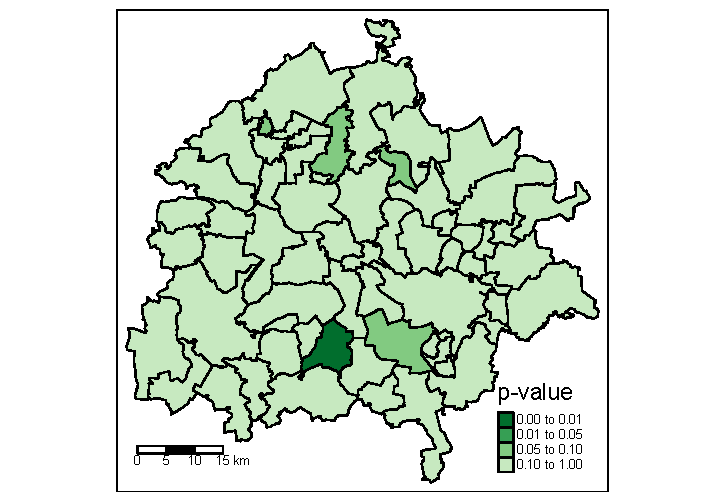
\includegraphics[scale=0.75,trim={0.2cm 0.1cm 0.2cm 0.1cm},clip]{body/figures/analysis/metropol-pval.pdf}% [scale=0.5] oder [width=\linewidth]
   %\caption{km2}
\end{minipage}
   %Source:
\caption[Lokale Autokorrelation]{Lokaler Moran Index: Li: Art der Korrelation. Re: Signifikanz. }
\label{fig_metropol_LMI}
\end{figure}


Zur detaillierten Untersuchung lokaler Autokorrelation eignet sich das Moran Scatterplot. 
Die Untersuchungsvariable  wird auf der x-Achse (Abszisse) dargestellt und die 
räumlich gewichteten, mittleren Nachbarwerte (engl. spatially lagged values) mittels y- Achse (Ordinate). 
Der globale Moran Index wird als linearer Zusammenhang zwischen beiden Größen durch den Anstieg 
einer hervorgehobenen Geraden dargestellt. Der Plot wird zudem an Position der beiden 
Erwartungswerte in vier Quadranten zerlegt. Diese klassifizieren alle lokalen Beobachtungswerte 
entweder nach Clustern niedriger Werte (engl. Low-Low), nach Hot-Spots niedriger Werte(engl. Low-High), 
Hot-Spots hoher Werte (engl. High-Low) oder Clustern hoher Werte (engl. High-High).